La spécification \href{https://cesium.com/blog/2021/11/10/introducing-3d-tiles-next/}{3D Tiles Next}\footnote{https://cesium.com/blog/2021/11/10/introducing-3d-tiles-next/} de \href{https://cesium.com/}{Cesium}\footnote{https://cesium.com/} est une spécification open source permettant de visualiser des données géospatiales en 3 dimensions.

Pour pouvoir être utilisé, un dataset de données géospatiales doit être partitionné car il est souvent trop complexe pour nos ordinateurs de le traiter en entier. Cette spécification décrit comment le faire en organisant ces données en \textit{Tiles} et en \textit{Tilesets} pour pouvoir ensuite être fournies à un client tel que Cesium. Les Tiles, ou tuiles, contiennent toutes les informations nécessaires à décrire une portion d'une database dans un espace 3D comme par exemple un \textit{bounding volume} qui décrit le volume 3D de la tuile ou encore son \textit{content} qui contient l'objet 3D à afficher. Une Tile contient aussi une liste de Tile appellée \textit{children}. Un Tilesets possède diverses informations comme la version de la spécification utilisée mais aussi une liste de Tile tout comme les Tiles. Cette structure permet de diviser les données en une hiérarchie de Tiles en arbre, ce qui facilite la recherche et le traitement des données.

\begin{figure}[H]
    \centering
    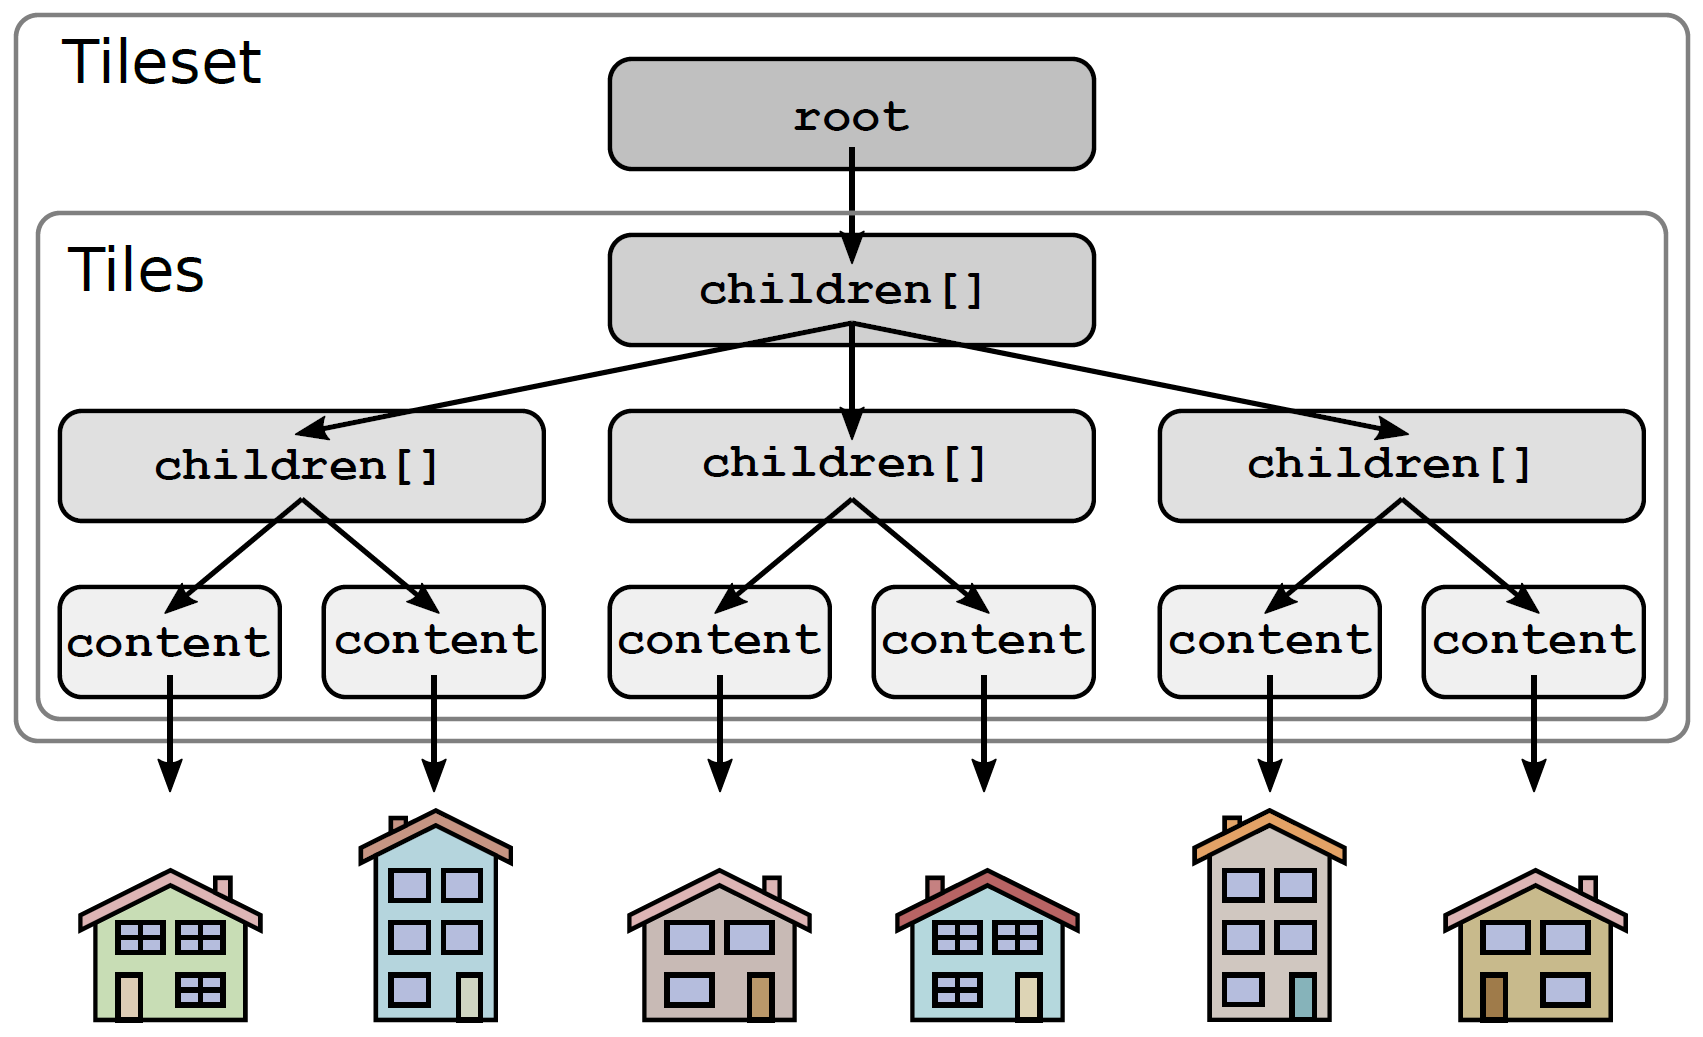
\includegraphics[width=0.6\textwidth]{assets/figures/Tilesets.png}
    \caption{Exemple de Tileset contenant un arbre de Tiles \cite{3d-tiles-reference-card-v1}}
    \label{fig:Tilesets}
\end{figure}

D'autres éléments sont présents dans les Tiles et Tilesets. Certains seront abordés plus tard dans ce rapport, sinon, pour plus d'informations sur la spécification 3D Tiles, vous pouvez consulter les \href{https://github.com/CesiumGS/3d-tiles/tree/main/reference-cards}{documents de références proposés par Cesium}\footnote{https://github.com/CesiumGS/3d-tiles/tree/main/reference-cards}.